\section{Partition Coloring Problem}

Let $G = (V, E)$ be a non-directed graph and $V$ partitioned into $q$ subsets $V_1, V_2,\ldots, V_q$, where $V_i \cap V_j = \emptyset, \forall i, j = 1, \ldots , q$, $i \neq j$. We refer to $V_1, V_2, \ldots , V_q$ as the components of the partition. The PCP consists in finding a subset $V' \subset V$ such that $|V' \cap V_i| = 1, \forall i = 1, \ldots , q$ (i.e., $V'$ contains one node of each component $V_i$), and the chromatic number of the graph induced in $G$ by $V'$ is minimum.\\
Figure \ref{pd:pcpExample} shows an example of an instance with $10$ nodes and a density of about $0.2$, where density is defined as the probability for each pair of nodes being connected by an edge.

\begin{figure}
\begin{center}
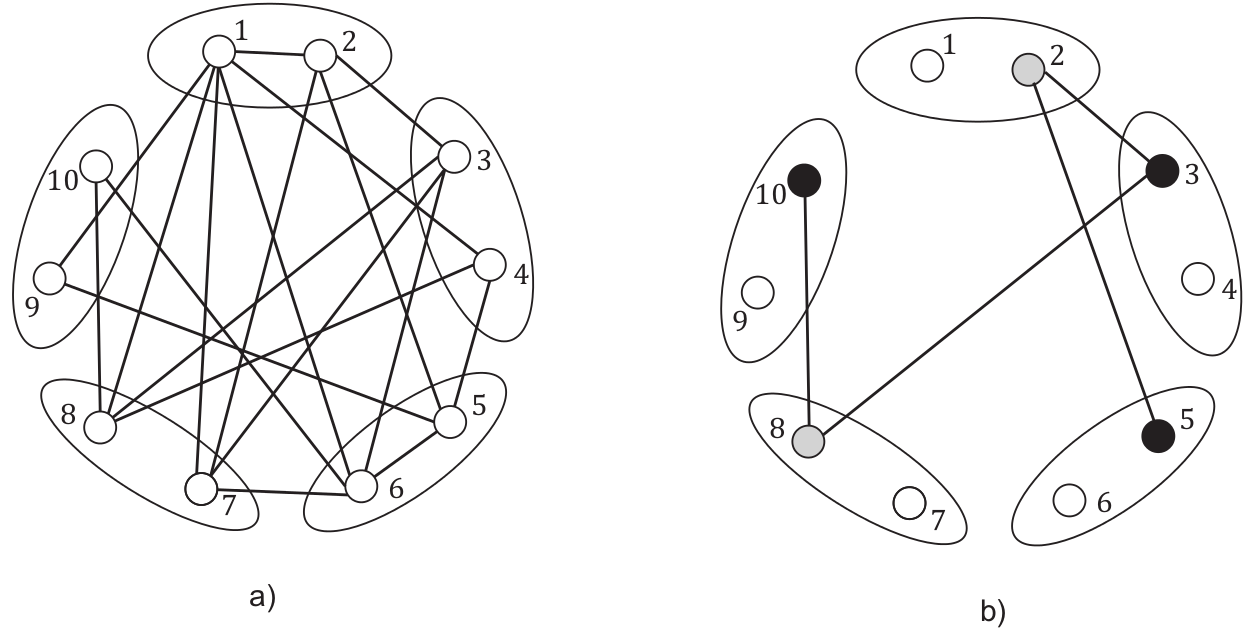
\includegraphics[scale=0.3]{figures/pcp.png}
\caption{(a) Shows a problem instance and (b) its solution.}
\label{pd:pcpExample}
\end{center}
\end{figure}


\section{Wavelength Routing and Assignment Problem}

The PCP has initially been considered by Li and Simha in \cite{li-00} and arises from considering the join problem of routing and wavelength assignment in WDM (Wavelength Division Multiplexing) optical networks. 

\section{Complexity}
This problem is clearly a generalization of the graph colouring problem. Li and Simha \cite{li-00}	
have shown that the decision version of PCP is
NP-complete.


